\chapter{Verification}
\section{Instruction decoding}
This sub-unit was tested along with the rest of the pipeline, since several signals coming from other stages are important to determine the control flow. For instance, the misprediction flag is generated in the MEM stage and the data used by the hazard detection unit comes from the pipeline registers. The instruction decoding stage was connected to a behavioral ALU in order to focus the debugging effort on the instruction sequence. \autoref{fig:wave} shows the occurrence of a branch (at $t=1.2\, \mu$s), the corresponding jump due to the taken prediction and the subsequent recovery two clock cycles later, when the prediction is found to be incorrect.

\begin{figure}
	\makebox[\textwidth][c]{
	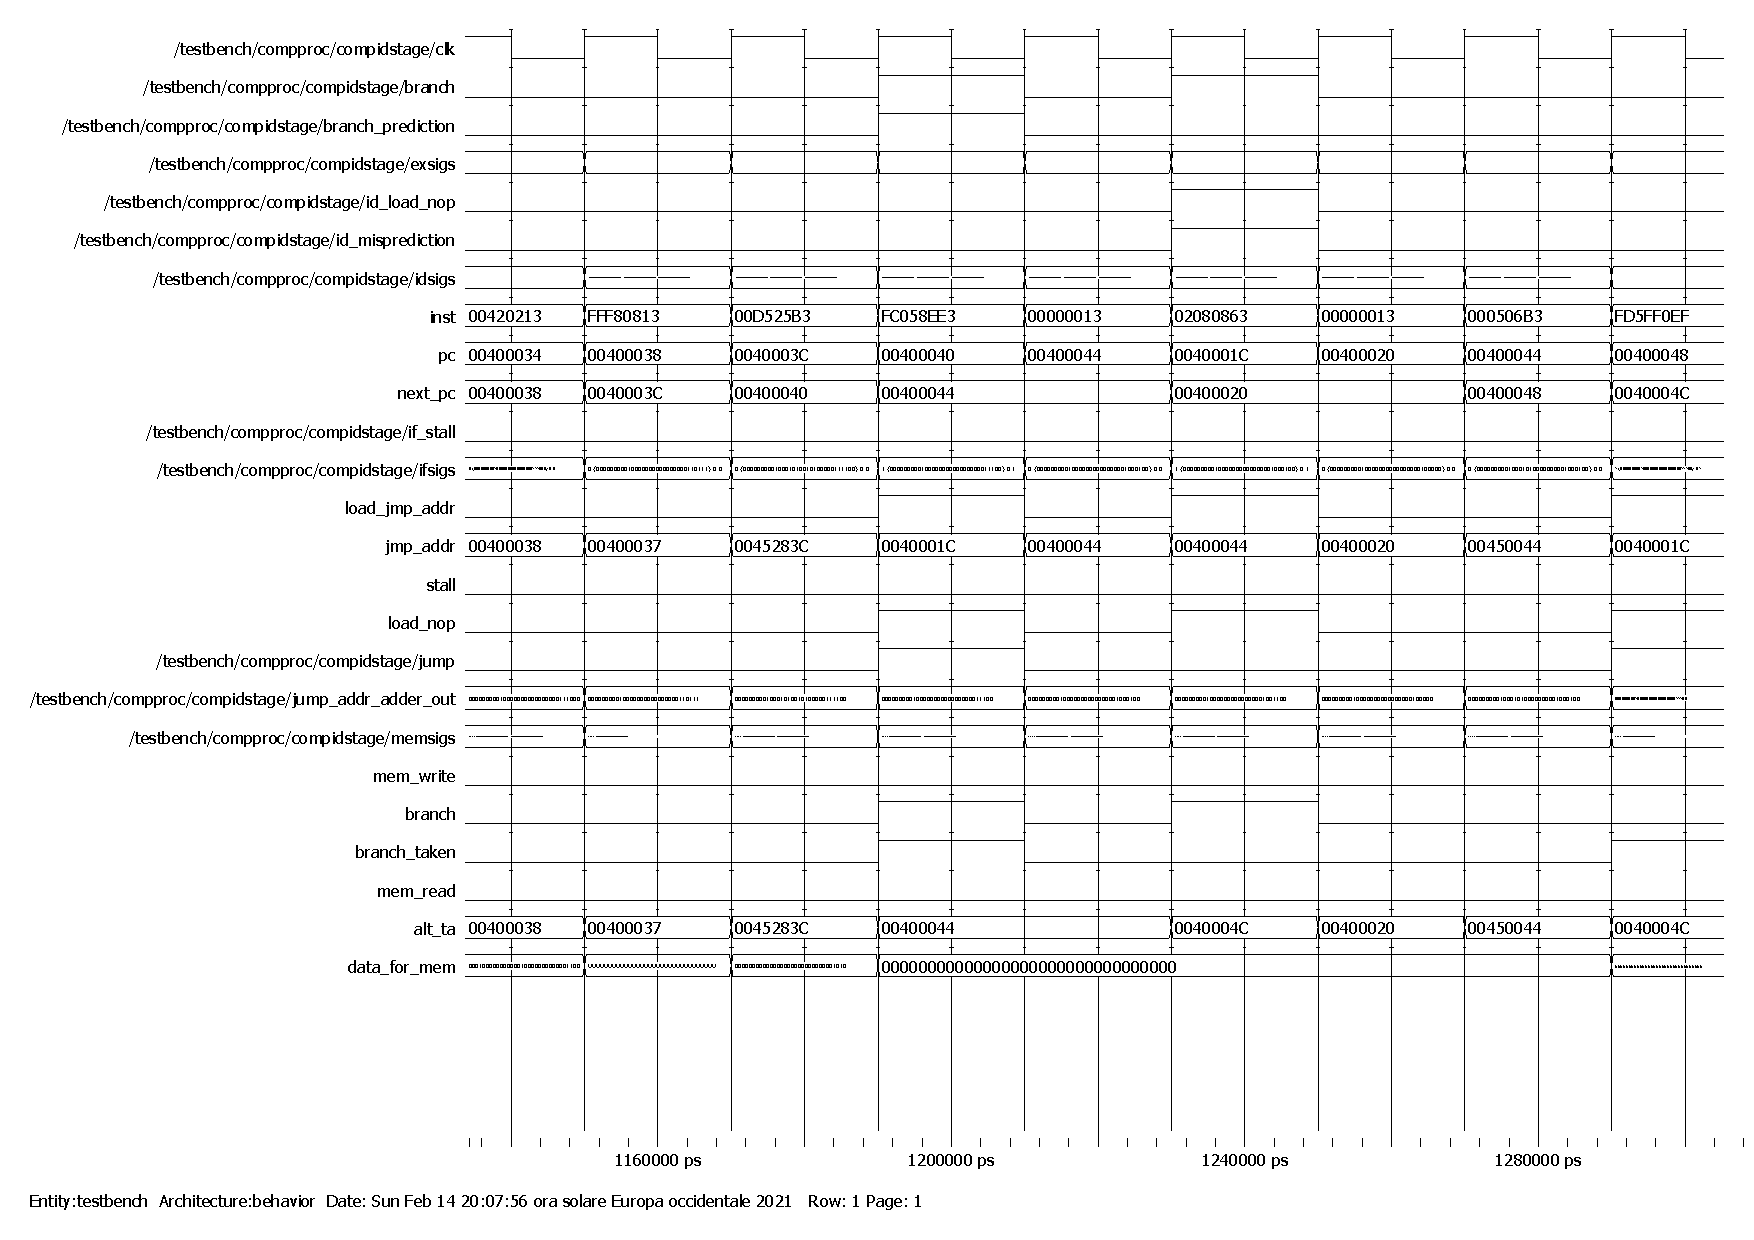
\includegraphics[angle=90, width=1.2\textwidth]{./images/wave.pdf}}
	\caption{Instruction decoding stage signals showing the occurrence of a branch and the following flush due to its misprediction.}
	\label{fig:wave}
\end{figure}


\section{Execution Stage}
The most significant component to verify is the ALU.

\newpage

\section{Testbench}
The testbench for the entire processor is made up of a testbench entity that instantiates the DUT along with a non-synthesizable memory component. This component loads the contents of the instruction and the data memory from a text file (hexadecimal text) at startup and provides address and data ports for the processor to read/write data. Moreover, it is capable of dumping the entire content of the data memory in a file to be compared with the correct result at the end of execution. This can be done at any time during the execution by asserting an input signal \texttt{dump}.

The program used for testing was the minimum search in a vector. Since the internal components had been singularly
tested, at this level it was more important to monitor the overall behavior and evolution of the system. Given the
high complexity of the system, the best solution was to test it by hand. After launching the simulation, the
dumped results were compared with the ones produced by the reference software, and once these were confirmed to be
correct, a manual check of the evolution of the system - in particular, the internal registers in the register file
and the program counter - step by step was done through Modelsim.

Naturally it was important to keep in mind that the reference software (which was not written from us) and may behave
slightly differently, for example branch prediction or forwarding may be structured differently.

Overall, the processor has shown the correct behavior and generated the expected results.
